\begin{frame}{Helpful Place Labels}
\vspace{-20pt}
\begin{figure}[htb!]
    \centering
    \includegraphics[width=0.85\linewidth]{../surge/plots/point_choosing/standard_loc_test.pdf}
    \vspace{-7pt}
    \caption{Places that I will label the x-axis with.
     The coastline is a self-similar fractal~\cite{mandelbrot1967long, richardson1961problem},
      hence coast length is dependent on resolution.
    [Fractal dimension changes along the coast.~\cite{jiang1998fractal}]}
    \label{fig:}
\end{figure}
\end{frame}


\begin{frame}[fragile]{Automatic Point Selection}
\vspace{-20pt}

\begin{algorithm}[H]
\dontprintsemicolon
% \DontPrintSemicolon % Some LaTeX compilers require you to use \dontprintsemicolon instead
\caption{Coastal Selection}
\label{algo:Selection}
\KwIn{Grid: boolean grid (True for NaN values (land))}
\For{indices in Grid}{
  \If {Grid[indices] == False}{
     \If{ any of Grid[index\_x $\pm$ 1, index\_y $\pm$ 1] are True}
        {\textbf{append} indices to List\;}
     }
}
\KwOut{List: list of indices}
\end{algorithm}

\end{frame}

\begin{frame}[fragile]{Automatic Point Sorting}
\vspace{-20pt}
\begin{algorithm}[H]
\dontprintsemicolon
% \DontPrintSemicolon % Some LaTeX compilers require you to use \dontprintsemicolon instead
\caption{Coastal Sort}
\label{algo:Sort}
\KwIn{Input\_List: Slimmed output of Algorithm~\ref{algo:Selection}}
\KwIn{First\_Index\_Pair: Point at one end of the coast }
\KwIn{Final\_Index\_Pair: Point at other end of the coast }

\texttt{tmp} $\gets$ First\_Index\_Pair\;

\Repeat{\texttt{tmp} = Final\_Index\_Pair}{
 \textbf{append} \texttt{tmp} to Output\_List\;
 \textbf{remove} \texttt{tmp} from Input\_List\;
 \texttt{tmp} $\gets$ Input\_List[\textbf{min}$_{k}$(\textbf{distance}(\texttt{tmp}, Input\_List[k]))]\;
}
\textbf{append} Final\_Index\_Pair to Output\_List\;

\KwOut{Output\_List: sorted list of indices}
\end{algorithm}

\end{frame}


\begin{frame}{Automatically Point Selection from ORCA12}
\vspace{-20pt}
\begin{figure}[htb!]
    \centering
    \hspace{-10pt}
    \includegraphics[width=0.60\linewidth]{../surge/plots/quiver_plot.pdf}
    \hspace{5pt}
    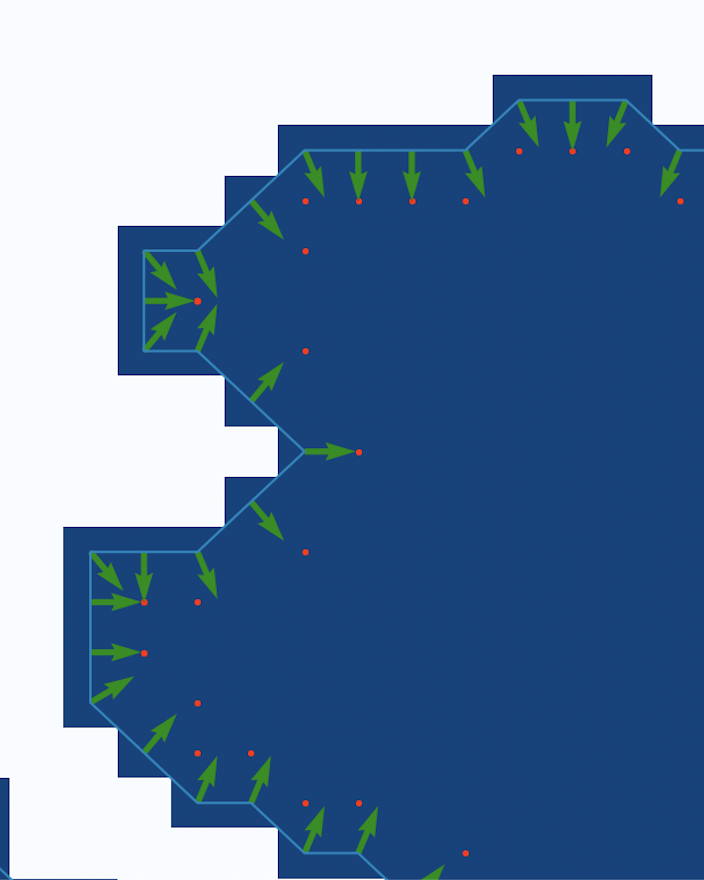
\includegraphics[width=0.38\linewidth]{images/example-images/new-orleans-example.png}
    \vspace{-7pt}
    \caption{The full selection of coastal points taken from ORCA12. Green arrows show
             orientation of that cell's stretch of coast line.}
    % \label{fig:}
\end{figure}
\end{frame}

\section{Local Coastal Metrics}
    \begin{frame}[plain]
        \vfill
      \centering
      \begin{beamercolorbox}[sep=8pt,center,shadow=true,rounded=true]{title}
        \usebeamerfont{title}\insertsectionhead\par%
        \color{oxfordblue}\noindent\rule{10cm}{1pt} \\
        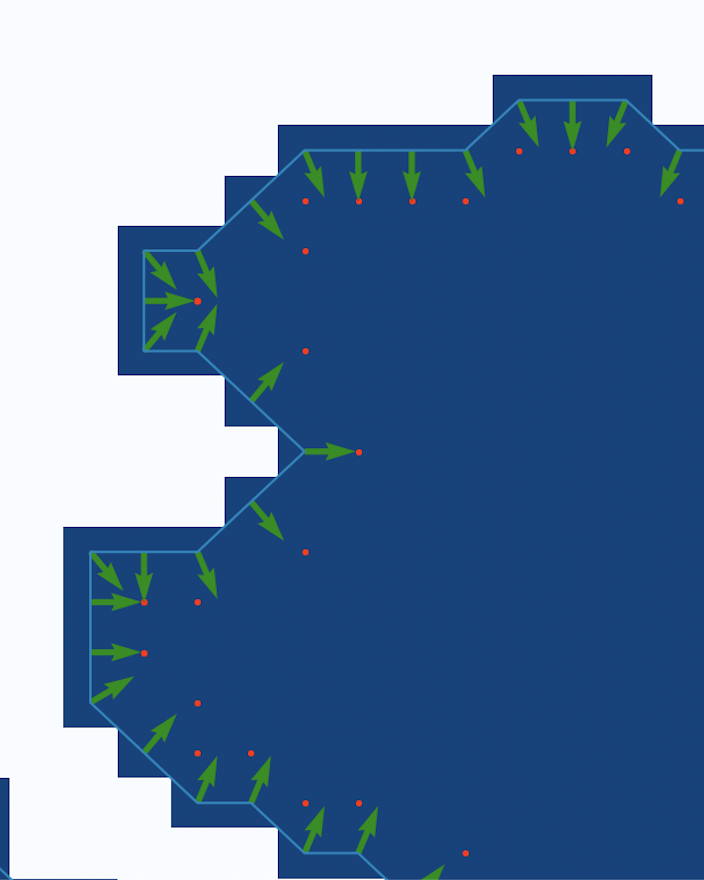
\includegraphics[width=0.4\linewidth]{images/example-images/new-orleans-example.png}
        \includegraphics[width=0.52\linewidth]{../surge/plots/angles_hist.pdf}
      \end{beamercolorbox}
      \vfill
  \end{frame}


\begin{frame}{The change in angles along the coastline}
\vspace{-20pt}
\begin{figure}[htb!]
    \centering
    \begin{equation}
B_i^{\prime}=\operatorname{arctan} 2\left(\sum_{j=i-4\sigma}^{j=i+4\sigma}
     \mathcal{N}(i, \sigma^{2})\cdot \sin{( B_{j})},\; \sum_{j=i-4\sigma}^{j=i+4\sigma}
      \mathcal{N}(i, \sigma^{2})\cdot  \cos{( B_{j})}\right)
\end{equation}
    \includegraphics[width=1.0\linewidth]{../surge/plots/angle_heatmap.pdf}
    % \caption{To deal with this we could smooth, and try a variety of $\sigma$.}
    % \label{fig:}
\end{figure}
\end{frame}


\begin{frame}{Angular derivative signal noisy for small $\sigma$}
\vspace{-20pt}
\begin{figure}[htb!]
    \centering
        \begin{equation}
        \frac{\partial B_i^{\prime}}{\partial \mathrm{pt}} \equiv \frac{B_{i+1}^{\prime}-B_{i-1}^{\prime}}{2}
\end{equation}
    \includegraphics[width=1.0\linewidth]{../surge/plots/derivative_heatmap_1_11.pdf}
    % \caption{To deal with this we could smooth, and try a variety of $\sigma$.}
    % \label{fig:}
\end{figure}
\end{frame}

%    plot_derivative_angle_heatmap(1, 11)
%    plot_derivative_angle_heatmap(10, 30)
%    plot_derivative_angle_heatmap(30, 100)

\begin{frame}{Better for  moderate $\sigma$}
\vspace{-20pt}
\begin{figure}[htb!]
    \centering
            \begin{equation}
        \frac{\partial B_i^{\prime}}{\partial \mathrm{pt}}
        \equiv \frac{B_{i+1}^{\prime}-B_{i-1}^{\prime}}{2} \notag
\end{equation}
    \includegraphics[width=1.0\linewidth]{../surge/plots/derivative_heatmap_10_30.pdf}
    % \caption{To deal with this we could smooth, and try a variety of $\sigma$.}
    % \label{fig:}
\end{figure}
\end{frame}

\begin{frame}{Unresponsive for high $\sigma$}
\vspace{-20pt}
\begin{figure}[htb!]
    \centering
\begin{equation}
        \frac{\partial B_i^{\prime}}{\partial \mathrm{pt}}
        \equiv \frac{B_{i+1}^{\prime}-B_{i-1}^{\prime}}{2} \notag
\end{equation}
    \includegraphics[width=1.0\linewidth]{../surge/plots/derivative_heatmap_30_100.pdf}
    % \caption{To deal with this we could smooth, and try a variety of $\sigma$.}
    % \label{fig:}
\end{figure}
\end{frame}


\begin{frame}{Extracting Bathymetry}
\vspace{-30pt}
\hspace{-30pt}
\begin{figure}[htb!]
    \centering
    \hspace{-30pt}\includegraphics[width=1.1\linewidth]{../surge/plots/bath_list.pdf}
    % \label{fig:}
\end{figure}
\end{frame}


\begin{frame}{Extracting Bathymetry}
\vspace{-30pt}
\hspace{-30pt}
\begin{figure}[htb!]
    \centering
    \hspace{-35pt}\includegraphics[width=1.1\linewidth]{../surge/plots/distance_isobath.pdf}
    % \label{fig:}
\end{figure}
\end{frame}

\begin{frame}{Isobath Distances are Heavily Correlated}
\vspace{-30pt}
\hspace{-30pt}
\begin{figure}[htb!]
    \centering
    \hspace{-35pt}\includegraphics[width=0.65\linewidth]{../surge/plots/isobath_correlate.pdf}
\end{figure}
\end{frame}

\begin{frame}{An Example around New Orleans}
\vspace{-30pt}
\begin{figure}[htb!]
    \centering
    \includegraphics[width=0.75\linewidth]{../surge/plots/new_orleans_map.pdf}
\end{figure}
\end{frame}

\begin{frame}{A Katrina-Like Hurricane}
\vspace{-30pt}
\begin{figure}[htb!]
    \centering
    \includegraphics[width=0.75\linewidth]{../surge/plots/katrina_graph.pdf}
\end{figure}
\end{frame}
